\chapter{System Evaluation}

\section{System Usability}
When Vertex was under research before development had begun the development team wanted the application to be functional and inclusive. In an attempt to make the application as easy to use, Flutter material components and Icons were used to develop a user interface that was aesthetically pleasing, easy to understand and functional. Flutters SDK was perfect for building out the core user interface components, its use of Widgets and OOP make it seamless to create, reuse and scale for components for different platforms. When a user is logged in they are greeted with the home page were they can see a list of channels they can interact with to communicate via text message, voice or video with other users in that channel. Figure ~\ref{image:convertionView} displays a text channel were user communicate via text messages.

\begin{figure}[h!]
    \caption{Conversation View}
    \label{image:convertionView}
    \centering
    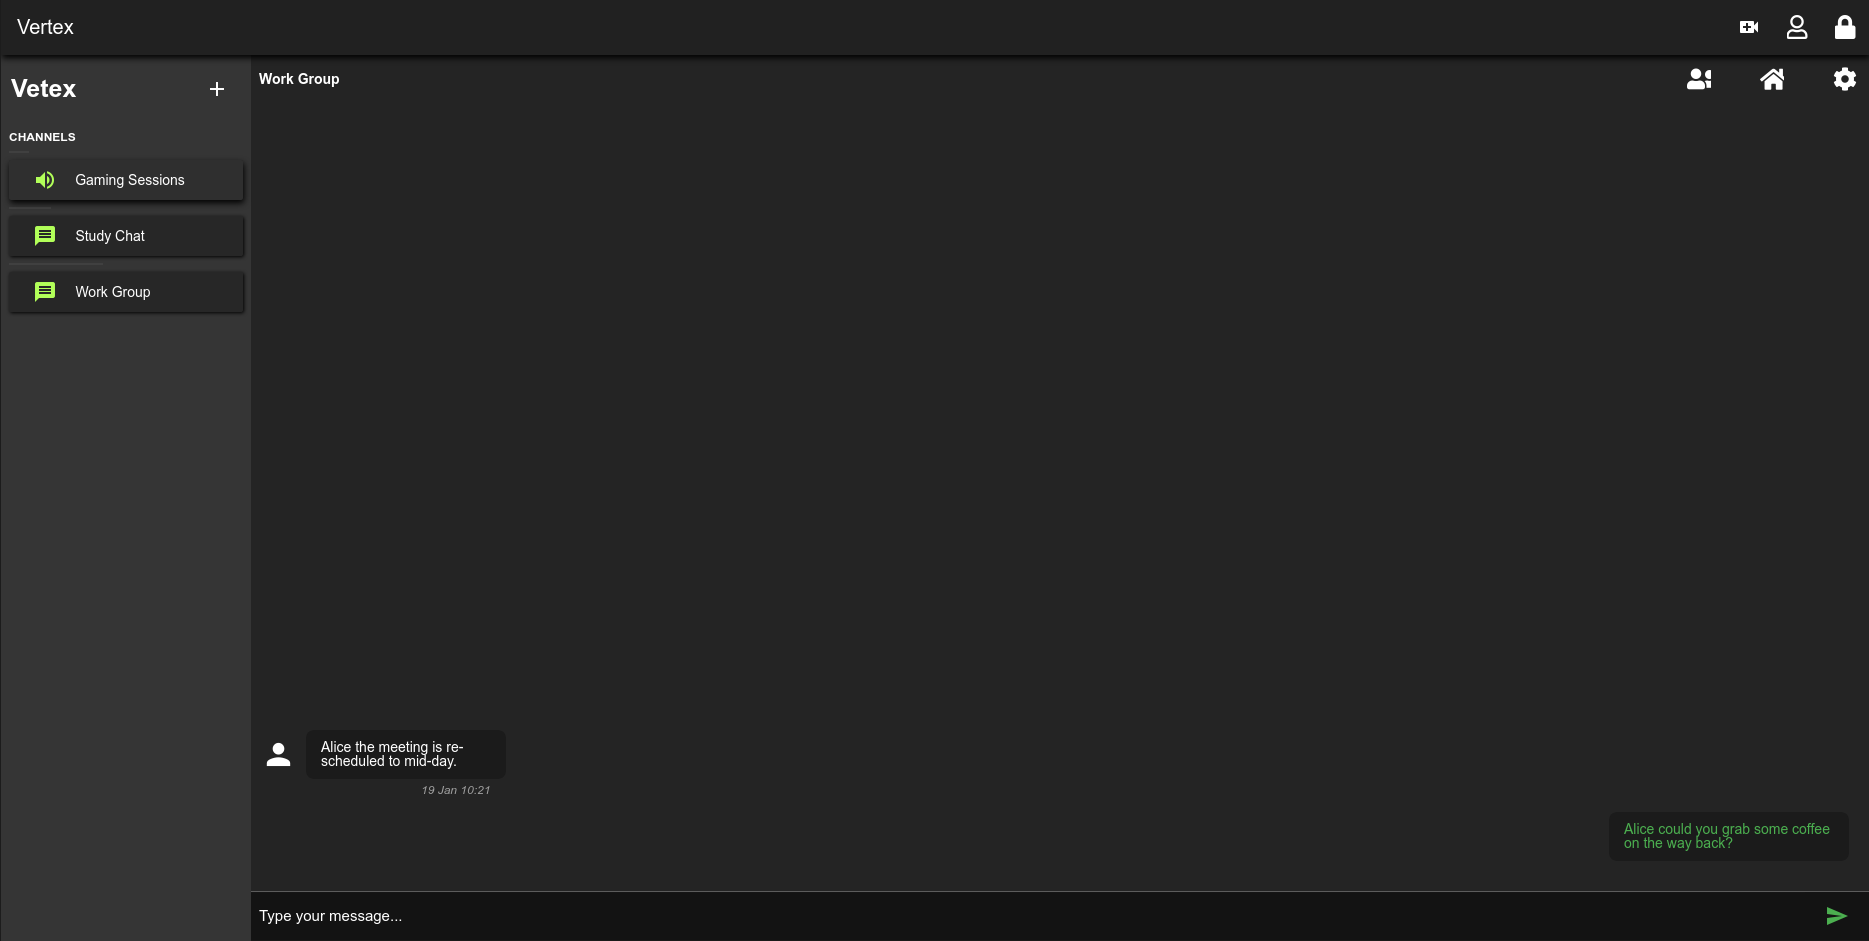
\includegraphics[width=0.8\textwidth]{images/screenshotsOfPages/conversationScreen.png}
\end{figure}

When a user wants to start a voice call with somebody they select a voice channel that is denote by a speaker icon next to the channel name in the list of channels where then a list of available users in that channel are available to communicate, to start a call all a user has to do is click on a user displayed in the list and it will connect the call with them. An example of the list of users in a voice channel can be seen in figure~\ref{image:voiceLobbyView}

\begin{figure}[h!]
    \caption{WebRTC Voice lobby}
    \label{image:voiceLobbyView}
    \centering
    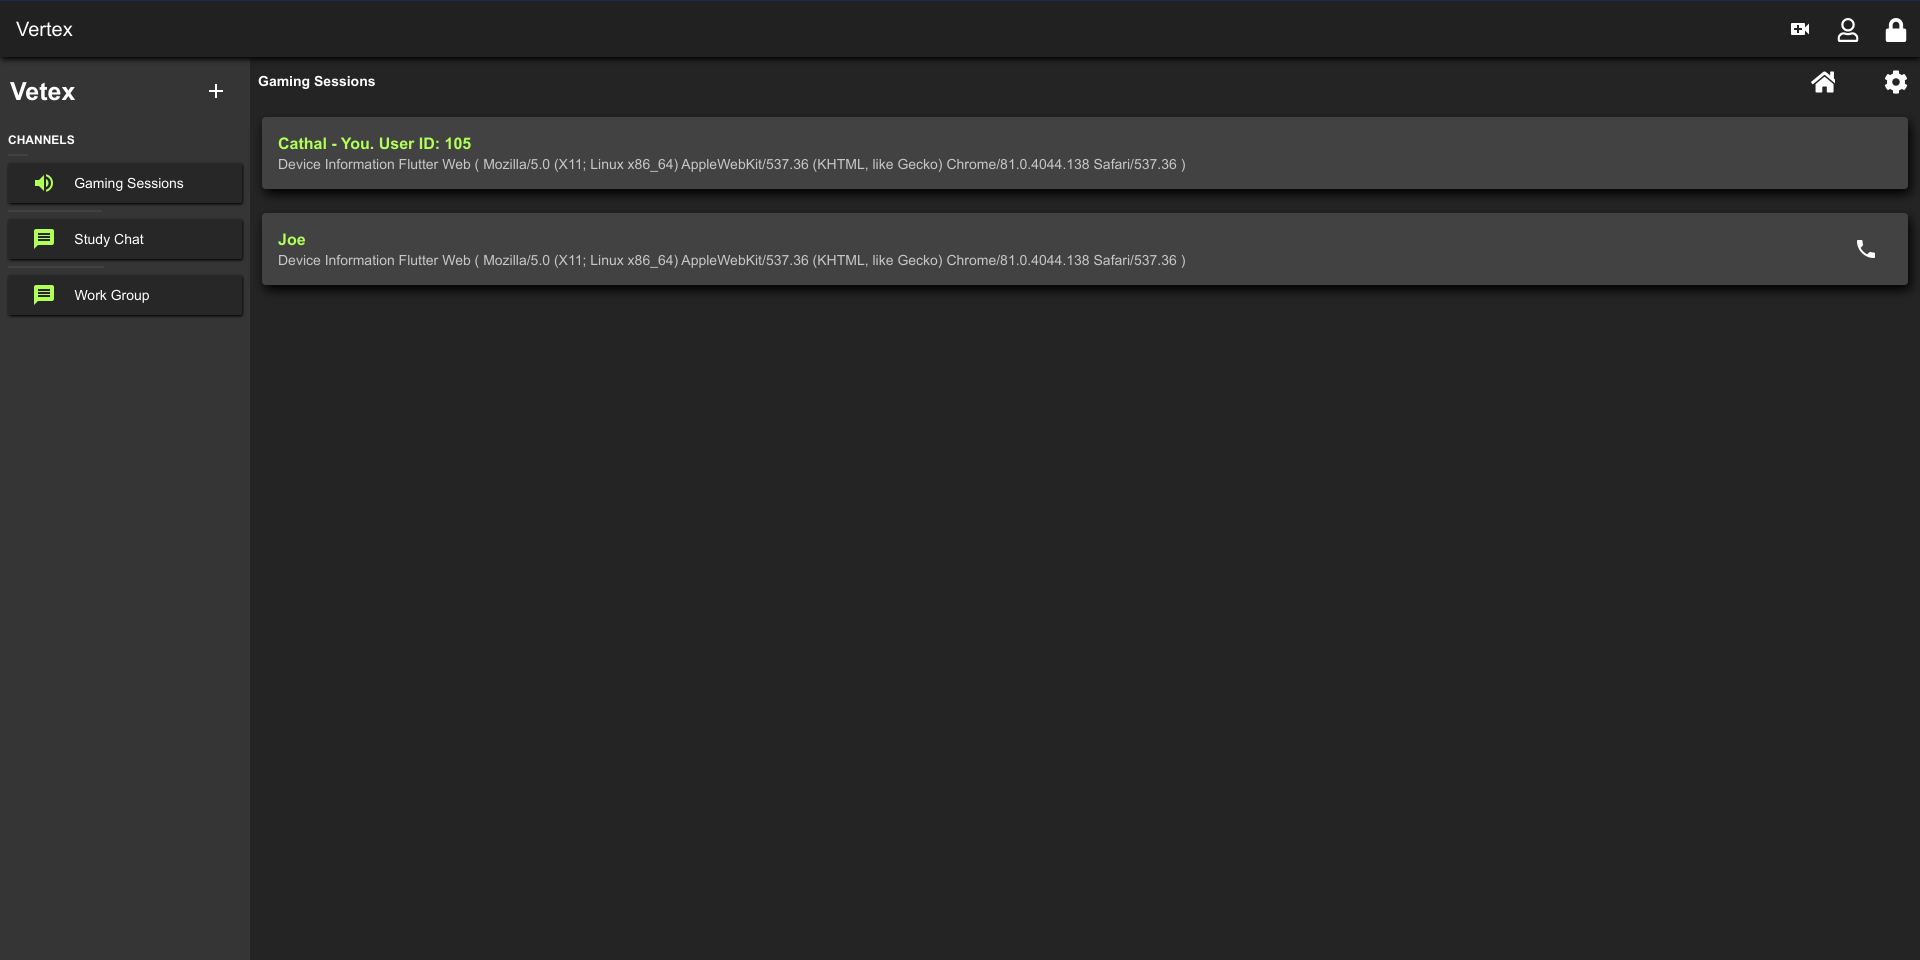
\includegraphics[width=0.8\textwidth]{images/screenshotsOfPages/voiceCallLobby.png}
\end{figure}

When a user wants to start a video call with another user they select the camera icon on the top right were it will also display a list of available users that wish to communicate. Once a user is selected and the call is set up the application will display the in call UI displaying the remote and local users video stream as seen in figure ~\ref{image:videoCall}

\begin{figure}[h!]
    \caption{WebRTC Video call}
    \label{image:videoCall}
    \centering
    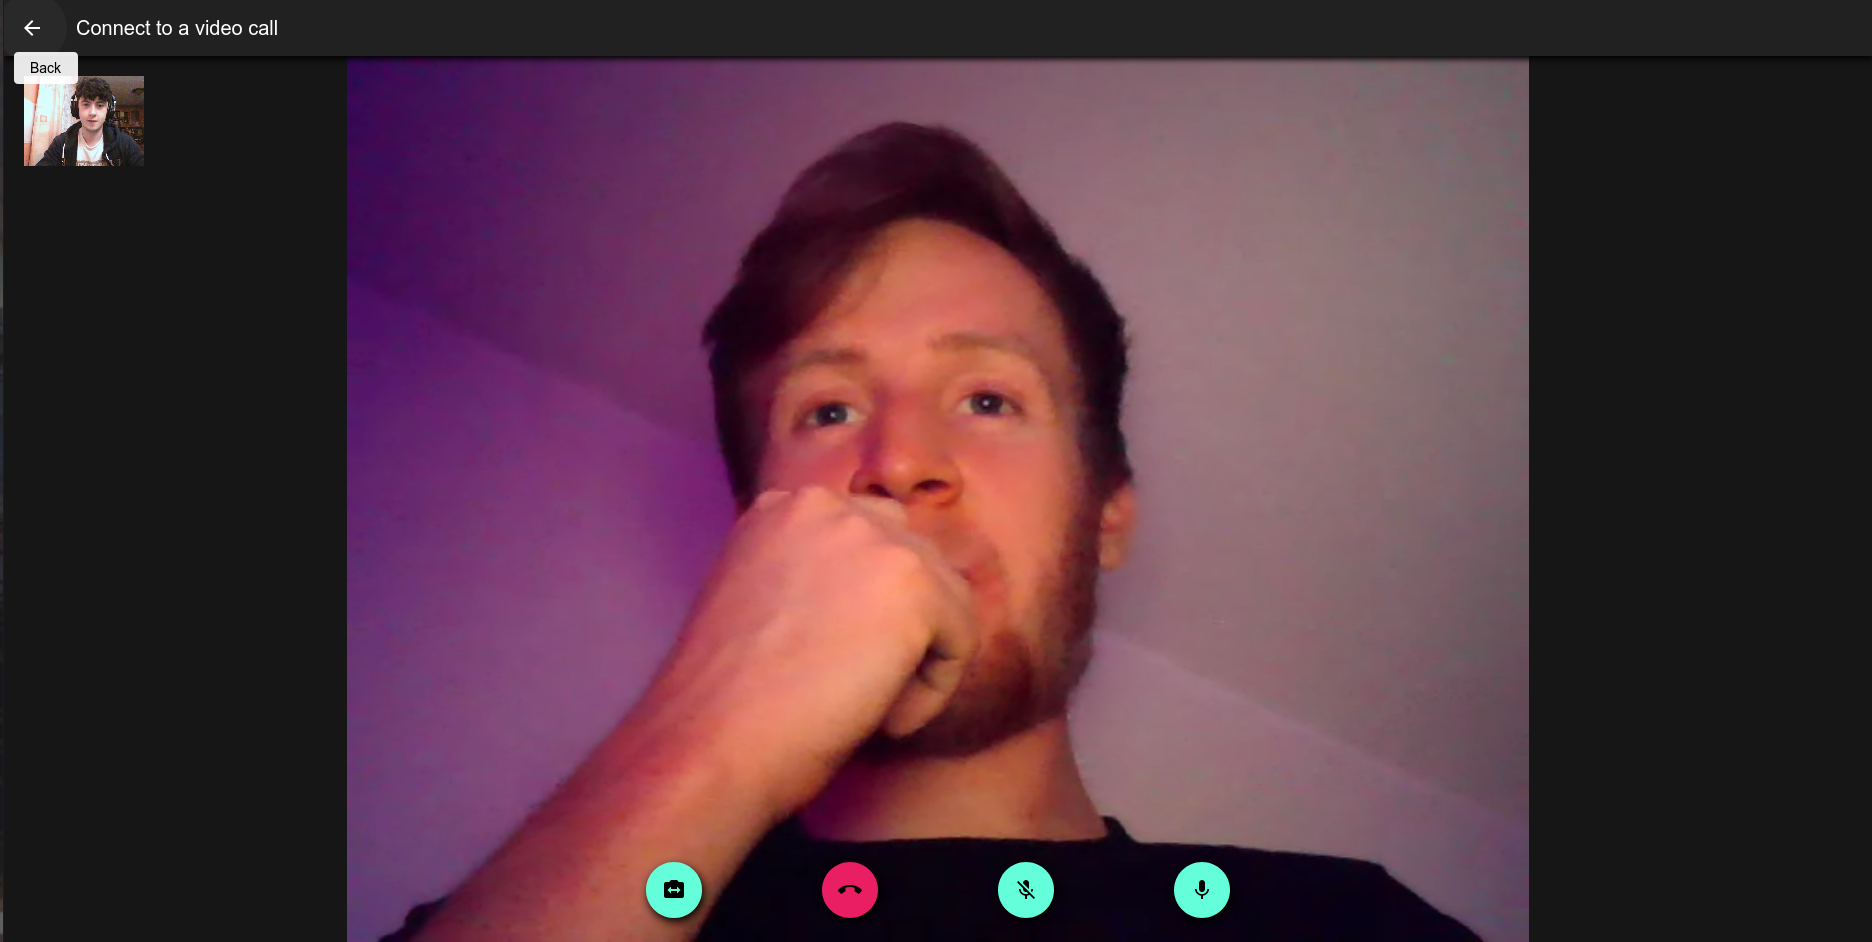
\includegraphics[width=0.8\textwidth]{images/screenshotsOfPages/webRTCProof2.png}
\end{figure}

\section{Robustness}
During the development of any project there comes a points were run-time exceptions and user error needs to be handled by the application. This can vary from invalid input from a user to a server that the application relies on not being online or currently unavailable. Below will break down the main areas were potential weak spots occur.

\subsection{Signalling Server}
As previously discussed in section~\ref{signallingTechR} WebRTC relies on a signalling server as peers need to send there session description which specifies the information on transport as well as media type. The signalling server is an external service away from the local client so it is possible the server could be offline or not reachable. To manage the applications state if this happens occurs
a SignallingState is returned from the application's web socket to the view letting the view know that it would display a message to the user that the server is not available. Figure~\ref{image:connectionError} displays an example of the error

\begin{figure}[h!]
    \caption{Connection Error}
    \label{image:connectionError}
    \centering
    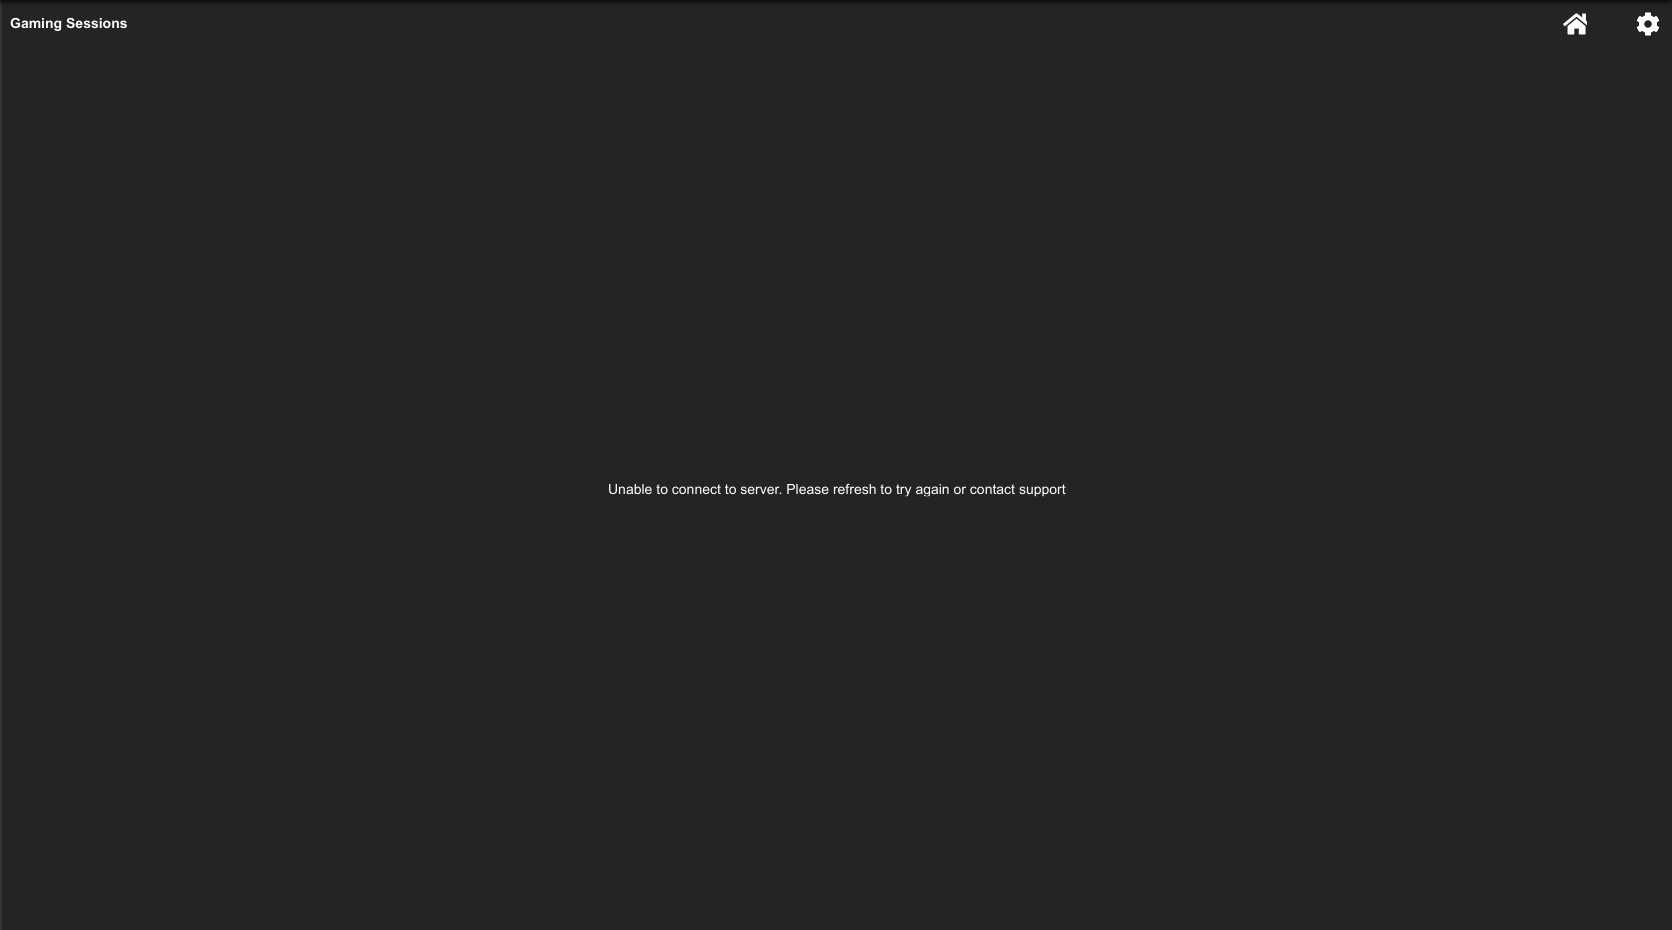
\includegraphics[width=0.8\textwidth]{images/screenshotsOfPages/connectionError.png}
\end{figure}

\section{Issues Encountered}
There were a number of issues that occurred during the development project. This section will break down some of the cores issues and how they were dealt with. 

\subsection{WebRTC}
WebRTC was a massive implementation in the project and a lot of time was spent to get it to were it is now. The WebRTC signalling server firstly needed to be developed so the client could connect to it to send and receive messages. Once the protocol has been set up correctly on the signalling server testing begun to try and get two peer to exchange session description data so they could create a connection to one another. This process did not go very well at the beginning and days were spent trying to figure out why a remote peer was unable to set the description of the connecting peer. It wasn't until a testing tool was found that is built into Google Chrome the browser to help debug WebRTC sessions. This tool can be found when you navigate to "chrome://webrtc-internals" in the search bar. With the help of the debugging tool the issued was tracked down to the ICE candidate information not actually getting delivered correctly to the remote peer. It turned out to be a issue with ids that are assigned to connections on the signalling server. In figure~\ref{image:webrtcDebugTool} an example is displayed of the tool


\begin{figure}[h!]
    \caption{WebRTC Debugging Tool}
    \label{image:webrtcDebugTool}
    \centering
    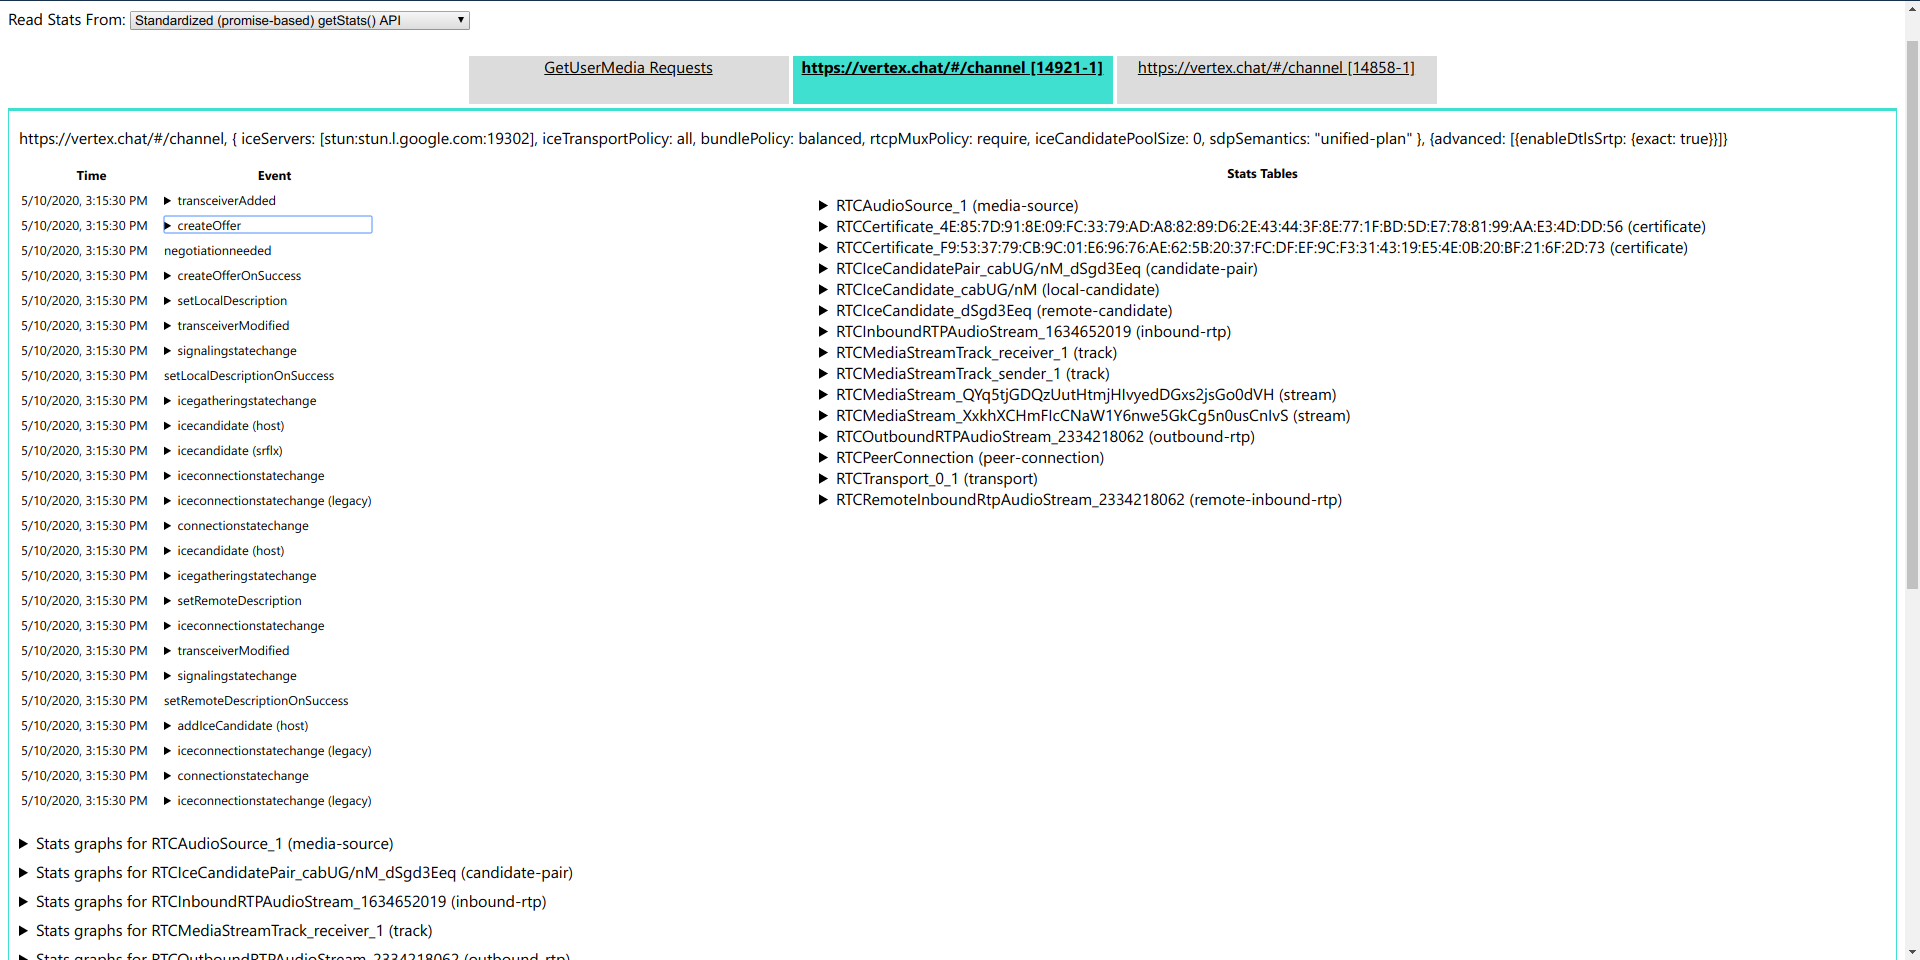
\includegraphics[width=0.8\textwidth]{images/screenshotsOfPages/webrtcTestingTools.png}
\end{figure}


In figure~\ref{image:webrtcDebugToolConnected} it demonstrates that the remote description has been set and the connection state is "connected" mean both peers are now communicating directly.   


\begin{figure}[h!]
    \caption{WebRTC Debugging Tool}
    \label{image:webrtcDebugToolConnected}
    \centering
    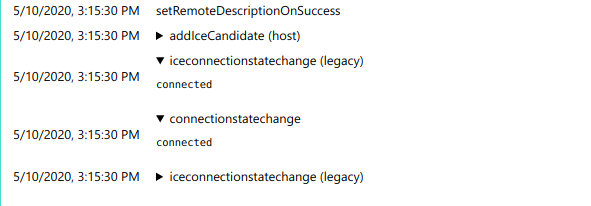
\includegraphics[width=0.8\textwidth]{images/screenshotsOfPages/webrtcTestingToolConnected.png}
\end{figure}

Another issue encountered when once peers were able to connect to each other was were the local users microphone was also playing back to them as well as the remote uses causing really bad echo on the line, unfortunately this issue was never rectified as the problem was unable to be solved up until project submission. 

% The application was initially going to include multi user voice call but due to time restrictions it was not possible to have it implemented in time but it is definitely possible in further development. 


\subsection{Platforms and Dart Packages}
Developing the application up till the final two weeks an issue was discovered with cookies and is believed to relate to CORS. When a session id was issued from the server on login the client browser would display the Set-Cookie in the header and also display it in the response of other requests made by the client so a user was authenticated each time with the server. The client needs to capture this session id locally as it was meant to be used with the notification system(as talked about in selection...). When printing the output of the headers client-side it did not hold the cookie or set-cookie value so the application was unable to store the session id rendering the possibility of connecting to the notification system dead. The real issues came when the application was tested on mobile devices where the device itself would not automatically handle the cookie like a browser would so even though the server was issuing the device a session id cookie the device was unable to return it to the server when a request was taking place. This quickly turned into a big issue that was causing a lot of headaches. When researching the issue it was suggested to use a different package for HTTP in Dart, like "request" or "dio" but both of there cookie manager packages did not support Flutter web and using them for mobile devices would require creating the API stubs for them again but that was not feasible. After a lot more research into the problem was carried out a solution was just not possible due to the remaining time restrictions. It was unfortunate as now the application will not run currently on mobile devices as it cant store the cookie and also the application on web cant store the session id cookie so that means the web build is unable to connect to the notification server.

